\documentclass[polish,envcountsect,10pt]{article}

   	\usepackage[T1]{fontenc}
   	\usepackage{polski}
    \usepackage{babel}
	\usepackage{subfigure}
	\usepackage{graphicx}
	\usepackage{geometry}
	\usepackage{listings}
	\usepackage{float}


	%\usepackage[hidelinks]{hyperref}
	
\title{Projekt badań oraz studium pilotażowe}
\author{prof. dr hab. inż. Chat GPT \and inż. Paulina Brzęcka 184701 \and inż. Marek Borzyszkowski 184266 \and inż. Wojciech Baranowski 184574}
\date{\today}
\begin{document}

\maketitle
\tableofcontents
\newpage

\section{Projekt badawczy}

\subsection{Tytuł}

Wykorzystanie obliczeń kwantowych w algorithmic trading.

\subsection{Opiekun}

Opiekunem projektu jest dr inż. Piotr Mironowicz.

\subsection{Cele i krótki opis}

Algorithmic trading, czyli handel algorytmiczny, to strategia inwestycyjna polegająca na wykorzystaniu zautomatyzowanych systemów handlowych do podejmowania decyzji inwestycyjnych na rynkach finansowych. Obliczenia kwantowe mają potencjał wzmocnienia tych strategii poprzez szybsze i bardziej efektywne przetwarzanie danych rynkowych oraz analizę trendów. W ramach tego tematu zostanie zbadana możliwość zaimplementowania agenta podejmującego decyzje inwestycyjne podczas gry na giełdzie, wykorzystując obliczenia kwantowe. Agent będzie testowany na emulatorze komputera kwantowego lub rzeczywistym komputerze, a jego skuteczność będzie porównywana z wybranymi algorytmami niekorzystającymi z technologii kwantowych. Efektem projektu będzie szkic artykułu naukowego opisującego przeprowadzone badania i wnioski z nich płynące.


\section{Projekt Badawczy}

\subsection{Cel badania}

\begin{itemize}
    \item Zbadanie potencjału obliczeń kwantowych w poprawie skuteczności strategii handlu algorytmicznego.
    \item Ocena możliwości implementacji agenta podejmującego decyzje inwestycyjne przy użyciu obliczeń kwantowych podczas gry na giełdzie.
    \item Porównanie skuteczności takiego agenta z wybranymi algorytmami niekorzystającymi z technologii kwantowych.
    \item Testowanie agenta na emulatorze komputera kwantowego lub rzeczywistym komputerze.
    \item Przygotowanie szkicu artykułu naukowego opisującego przeprowadzone badania i ich wyniki.
\end{itemize}

\subsection{Luka badawcza}

Temat badań został zformułowany w bardzo generalny sposób. Na obecny moment nie udało się zidentyfikować istotnych luk badawczych, gdyż definicja poszukiwanych wiadomości jest zbyt ogólna.

\subsection{Pytania badawcze}

\begin{enumerate}
    \item Czy agent podejmujący decyzje inwestycyjne oparty na obliczeniach kwantowych może wykazywać lepszą skuteczność w porównaniu z tradycyjnymi algorytmami?
    \item Jakie są różnice w skuteczności działania agenta opartego na obliczeniach kwantowych w porównaniu z algorytmami tradycyjnymi?
    \item Jakie są główne wyzwania związane z implementacją agenta wykorzystującego obliczenia kwantowe?
\end{enumerate}

\subsection{Hipotezy badawcze}

\begin{enumerate}
    \item 
        \begin{itemize}
			\item \textbf{Hipoteza zerowa:} Nie ma różnicy w skuteczności decyzji inwestycyjnych podejmowanych przez agenta opartego na obliczeniach kwantowych i tradycyjne algorytmy.
			\item \textbf{Hipoteza alternatywna:} Agent oparty na obliczeniach kwantowych wykazuje lepszą skuteczność w podejmowaniu decyzji inwestycyjnych niż tradycyjne algorytmy.
        \end{itemize}
        
    \item 
        \begin{itemize}
			\item \textbf{Hipoteza zerowa:} Nie ma istotnej różnicy w skuteczności działania agenta opartego na obliczeniach kwantowych w porównaniu z algorytmami tradycyjnymi.
			\item \textbf{Hipoteza alternatywna:} Skuteczność działania agenta opartego na obliczeniach kwantowych różni się istotnie od algorytmów tradycyjnych.
        \end{itemize}
        
    \item 
        \begin{itemize}
			\item \textbf{Hipoteza zerowa:} Nie ma istotnych wyzwań związanych z implementacją agenta wykorzystującego obliczenia kwantowe w praktyce na rynku finansowym.
			\item \textbf{Hipoteza alternatywna:} Istnieją istotne wyzwania związane z implementacją agenta wykorzystującego obliczenia kwantowe w praktyce na rynku finansowym.
        \end{itemize}
\end{enumerate}

\subsection{Podmioty badawcze} 

\begin{itemize}
	\item \textbf{Podmioty badawcze:} W naszym badaniu podmiotami badawczymi będą różne rodzaje instrumentów finansowych oraz ich zachowanie na rynkach. Może to obejmować akcje, obligacje, a także różne typy instrumentów pochodnych. Istotne będzie również uwzględnienie różnorodności sektorów rynku finansowego oraz różnych okresów czasowych, aby móc dokładnie zbadać wpływ obliczeń kwantowych na różne aspekty inwestycji.
    
	\item \textbf{Kryteria kwalifikacyjne:} Aby zapewnić odpowiednią reprezentatywność próbki oraz uniknąć wprowadzenia błędów do analizy, konieczne będzie określenie kryteriów kwalifikacyjnych dla wybranych podmiotów. Możemy uwzględnić takie czynniki jak stabilność instrumentu, płynność rynku, stopień złożoności instrumentu finansowego oraz historyczne dane dotyczące jego zachowania na rynku.
    
	\item \textbf{Metoda próbkowania:} W związku z dużą ilością danych rynkowych oraz różnorodnością instrumentów finansowych, konieczne będzie zastosowanie odpowiedniej metody próbkowania. W naszym badaniu możemy rozważyć techniki próbkowania losowego lub systematycznego, przy uwzględnieniu różnych sektorów rynku oraz różnych typów instrumentów finansowych. Istotne będzie również monitorowanie i ograniczenie wpływu błędów próbkowania na ostateczne wyniki analizy.
\end{itemize}

\subsection{Operacjonalizacja}

\begin{itemize}
	\item \textbf{Zmienne niezależne:}
    \begin{itemize}
        \item strategie handlowe (np. analiza techniczna, analiza fundamentalna),
        \item wskaźniki rynkowe (np. wskaźniki trendu, oscylatory),
        \item dane makroekonomiczne (np. wskaźniki gospodarcze, polityka pieniężna).
    \end{itemize}
	\item \textbf{Zmienne zależne:}
    \begin{itemize}
        \item stopa zwrotu,
        \item ryzyko inwestycji,
        \item skuteczność strategii handlowych.
    \end{itemize}
	\item \textbf{Zmienne zakłócające:}
    \begin{itemize}
        \item zmienność rynkowa,
        \item zmiany regulacyjne,
        \item błędy w danych rynkowych.
    \end{itemize}
    \item \textbf{Ukryte zmienne:}
    \begin{itemize}
        \item preferencje inwestorów,
        \item manipulacje rynkowe,
        \item ukryte czynniki ryzyka.
    \end{itemize}
\end{itemize}

\subsection{Metody badawcze}

\begin{itemize}
    \item \textbf{Eksperymenty kontrolowane}: Przeprowadzenie kontrolowanych eksperymentów, w których badane są różne strategie inwestycyjne oparte na obliczeniach kwantowych w porównaniu z tradycyjnymi strategiami. Eksperymenty mogą być realizowane w formie symulacji komputerowych, a następnie analizowane pod kątem skuteczności i efektywności strategii.
    
    \item \textbf{Studia przypadków}: Badanie konkretnych przypadków inwestycyjnych, w których agent inwestycyjny oparty na obliczeniach kwantowych jest testowany. Analiza poszczególnych przypadków pozwala na zdobycie szczegółowych wniosków na temat skuteczności strategii w różnych scenariuszach inwestycyjnych.
    
    \item \textbf{Analiza danych historycznych}: Badanie danych historycznych rynków finansowych i wyników różnych strategii inwestycyjnych w celu oceny skuteczności agentów opartych na obliczeniach kwantowych oraz przewidywania ich zachowania w przyszłości.
\end{itemize}

\subsection{Narzędzia badawcze}

\textbf{Plan Przeprowadzenia Symulacji:}
\begin{itemize}
	\item \textbf{Wybór platformy symulacyjnej:} wybór odpowiedniej platformy do przeprowadzenia symulacji komputerowych, uwzględniającej możliwość implementacji strategii opartych na obliczeniach kwantowych.
    
	\item \textbf{Implementacja strategii:} opracowanie strategii inwestycyjnych opartych na obliczeniach kwantowych oraz tradycyjnych strategii inwestycyjnych do zastosowania w symulacji.
    
	\item \textbf{Wybór scenariuszy rynkowych:} określenie różnorodnych scenariuszy rynkowych do symulacji, uwzględniających zmienność rynkową oraz różne warunki ekonomiczne.
    
	\item \textbf{Przeprowadzenie symulacji:} wykonanie symulacji komputerowych, w których zaimplementowane strategie są testowane w wybranych scenariuszach rynkowych.
    
	\item \textbf{Analiza wyników:} analiza wyników symulacji w celu oceny skuteczności oraz porównania efektywności strategii inwestycyjnych opartych na obliczeniach kwantowych z tradycyjnymi strategiami.
\end{itemize}

\noindent\textbf{Zakres Studium Przypadku:}
\begin{itemize}
	\item \textbf{Opis studium przypadku:} badanie konkretnego przypadku inwestycyjnego, w którym agent inwestycyjny oparty na obliczeniach kwantowych będzie testowany.
    
	\item \textbf{Wybór instrumentów finansowych:} Wybór różnych instrumentów finansowych do analizy w ramach studium przypadku, takich jak akcje, obligacje, opcje, czy inne instrumenty pochodne.
    
	\item \textbf{Analiza wyników:} analiza wyników inwestycyjnych uzyskanych przy użyciu agenta opartego na obliczeniach kwantowych w porównaniu z wynikami uzyskanymi przy użyciu tradycyjnych strategii inwestycyjnych.
\end{itemize}

\noindent\textbf{Plan Wykonania:}
\begin{itemize}
	\item \textbf{Przygotowanie:} przygotowanie środowiska symulacyjnego oraz danych historycznych rynkowych do przeprowadzenia symulacji.
    
	\item \textbf{Implementacja strategii:} implementacja strategii inwestycyjnych opartych na obliczeniach kwantowych oraz tradycyjnych strategii inwestycyjnych.
    
	\item \textbf{Przeprowadzenie symulacji:} wykonanie symulacji komputerowych z wykorzystaniem zaimplementowanych strategii w wybranych scenariuszach rynkowych.
    
	\item \textbf{Analiza wyników:} analiza uzyskanych wyników symulacji w celu oceny skuteczności oraz porównania efektywności strategii inwestycyjnych.
    
	\item \textbf{Raportowanie:} opracowanie raportu z wynikami symulacji oraz studium przypadku, zawierającego wnioski i rekomendacje dotyczące dalszych działań.
\end{itemize}

\subsection{Oczekiwane Wyniki}

\begin{itemize}
\item \textbf{Oczekiwane wyniki jakościowe:} Oczekiwane wyniki jakościowe obejmują ocenę efektywności nowych strategii inwestycyjnych w porównaniu z tradycyjnymi metodami, identyfikację potencjalnych korzyści wynikających z wykorzystania obliczeń kwantowych, analizę różnic w wynikach inwestycyjnych między różnymi instrumentami finansowymi oraz ocenę stabilności i spójności wyników symulacji w zróżnicowanych warunkach rynkowych.

\item \textbf{Oczekiwane wyniki ilościowe:} Oczekiwane wyniki ilościowe obejmują miary wydajności, takie jak procentowy zwrot z inwestycji, wskaźniki ryzyka, średnie zyski i straty, ilość transakcji wygenerowanych przez strategie inwestycyjne, a także inne metryki numeryczne, które mogą być wykorzystane do kwantyfikacji wyników analizy danych rynkowych.
\end{itemize}

\subsection{Zagrożenia wiarygodności}

\begin{itemize}

	\item \textbf{Wiarygodność konstrukcji:} Istnieje ryzyko, że definicje zmiennych, takich jak skuteczność strategii inwestycyjnych czy wyniki symulacji, mogą być niejasne lub nieprecyzyjnie zdefiniowane. Dodatkowo, sposób, w jaki te zmienne są mierzone, może być niejednoznaczny, co prowadzi do błędów w interpretacji wyników.

	\item \textbf{Wiarygodność wnioskowania:} Brak uwzględnienia wszystkich istotnych zmiennych lub niewłaściwe kontrolowanie zmiennych zakłócających może prowadzić do błędnych wniosków dotyczących przyczynowości między zmiennymi. Brak odpowiedniej kontroli eksperymentalnej lub randomizacji może pogłębić te zagrożenia.

	\item \textbf{Wiarygodność wewnętrzna:} Gdy nie można przeprowadzić realistycznych symulacji na rzeczywistym rynku finansowym, wiarygodność wewnętrzna może być zagrożona. Dodatkowo, niedostateczne dopasowanie grup eksperymentalnych i kontrolnych lub brak uwzględnienia wszystkich istotnych zmiennych mogą zakłócić wewnętrzną wiarygodność badania.

	\item \textbf{Wiarygodność zewnętrzna:} Istnieje ryzyko, że wyniki uzyskane z badań mogą mieć ograniczoną możliwość generalizacji na inne populacje inwestorów lub sytuacje rynkowe. Jeśli próba badawcza nie jest reprezentatywna dla ogólnej populacji inwestorów lub warunki symulacji różnią się od rzeczywistych warunków rynkowych, może to wpłynąć na zewnętrzną wiarygodność badania.
\end{itemize}

\subsection{Plan badawczy}

\begin{itemize}
    \item \textbf{Faza 1 (przygotowanie):}
    \begin{itemize}
        \item ustalenie celów projektu,
        \item określenie terminów projektu,
        \item utworzenie zespołu projektowego,
        \item przegląd literatury naukowej,
		\item zebranie danych potrzebnych do przeprowadzenia badania.
    \end{itemize}
    
    \item \textbf{Faza 2 (przeprowadzenie badania):}
    \begin{itemize}
        \item implementacja algorytmów i modeli klasycznych,
        \item implementacja algorytmów i modeli kwantowych,
        \item eksperymenty z użyciem obydwu modeli,
		\item porównanie rezultatów i wyciągnięcie wniosków,
        \item sporządzenie dokumentacji przeprowadzonego badania.
    \end{itemize}
    
    \item \textbf{Faza 3 (zakończenie projektu):}
    \begin{itemize}
        \item finalizacja dokumentacji,
        \item przygotowanie prezentacji projektu,
        \item przygotowanie materiałów do publikacji.
    \end{itemize}
\end{itemize}

\subsection{Cele publikacyjne}

\textbf{Możliwe publikacje:}

\begin{enumerate}
    \item \textbf{Artykuł badawczy:} Artykuł naukowy przedstawiający wyniki badania, wnioski i implikacje dla dziedziny algorytmicznego handlu i finansów. Artykuł ten mógłby zawierać opis teoretycznych podstaw badania, metodologię, uzyskane wyniki oraz dyskusję na temat znaczenia odkryć dla praktyki handlowej i dalszych badań.
    
    \item \textbf{Studium przypadku:} Publikacja opisująca szczegółowo przeprowadzone studium przypadku, w którym agent inwestycyjny oparty na obliczeniach kwantowych został testowany. Taka publikacja mogłaby zawierać opis wybranego przypadku inwestycyjnego, analizę wyników uzyskanych przy użyciu agenta kwantowego oraz porównanie z wynikami uzyskanymi przy użyciu tradycyjnych strategii inwestycyjnych.
    
    \item \textbf{Analiza teoretyczna:} Publikacja skupiająca się na analizie teoretycznej potencjalnych korzyści i ograniczeń związanych z algorytmicznym handlem opartym na obliczeniach kwantowych. Taka analiza mogłaby obejmować przegląd literatury, analizę matematyczną strategii inwestycyjnych oraz dyskusję na temat ich potencjalnego wpływu na rynek finansowy.
    
\end{enumerate}
\section{Studium Pilotażowe}

\subsection{Podmioty badawcze}

Wybranym badanym elementem będzie indeks S\&P500. Dane pozyskane z indeksu to będą odczyty notowań danego indeksu z jego zamknięcia danego dnia. Zakres rozpatrywanych dat to od 07 Marca 2023 do 07 Marca 2024 z odczytem dziennym. 

TU WSTAWIĆ INDEKS S\&P500

Do odpowiedniego porównania algorytmów klasycznych i kwantowych, zostaną wybrane algorytmy podobnego typu:
\begin{itemize}
    \item Algorytm genetyczny - dobieranie portfolio na wykorzystując działanie algorytmu genetycznego na komputerze klasycznym.
    \item Algorytm genetyczny z wykorzystaniem bramek kwantowych - dobieranie portfolio na wykorzystując działanie algorytmu genetycznego, gdzie dodatkowo dobór danej akcja w portfolio jest dodatkowo obciążony prawdopodobieństwem wynikającym z kwantowej natury wykorzystanych bramek.
\end{itemize}

\subsection{Realizacja Studium}

Każdy z algorytmów, nastawiony na jak największy zysk, zostanie przetestowany na wybranym przedziale czasowym danego indeksu. Ze względu na stochastyczną naturę obu z algorytmów, zostanie przeprowadzone 5 testów każdego z nich, a następnie do porównanie wykorzystany zostanie najlepszy z prób danego algorytmu.

\subsection{Wyniki}

\begin{figure}[H]
    \centering
    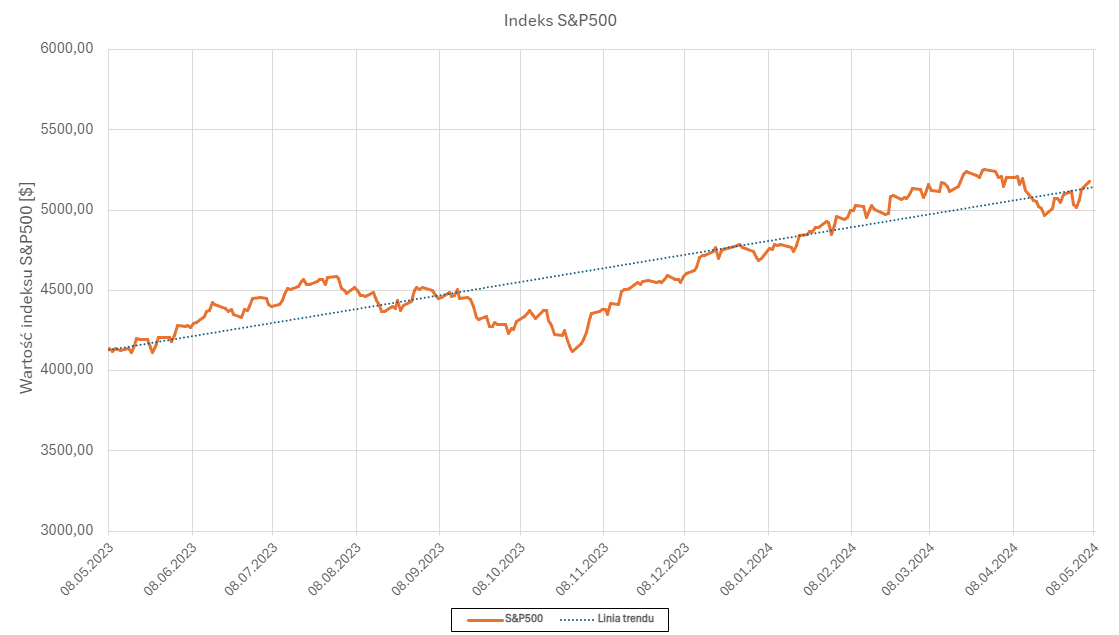
\includegraphics[width=0.8\textwidth]{SP500.png}
    \caption{Wyres indeksu S\&P500. }
    \label{fig:SP500}
\end{figure}

\begin{figure}[H]
    \centering
    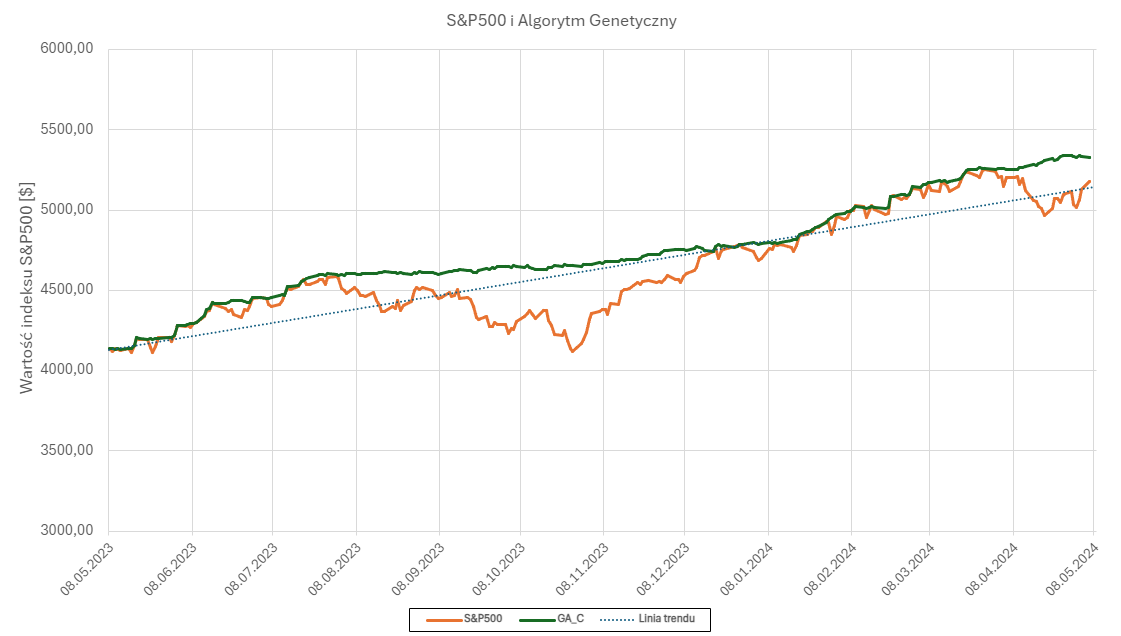
\includegraphics[width=0.8\textwidth]{GA_C.png}
    \caption{Zestawienie indeksu S\&P500 z graniem na giełdzie z wykorzystaniem algorytmu genetycznego. }
    \label{fig:GA_C}
\end{figure}

\begin{figure}[H]
    \centering
    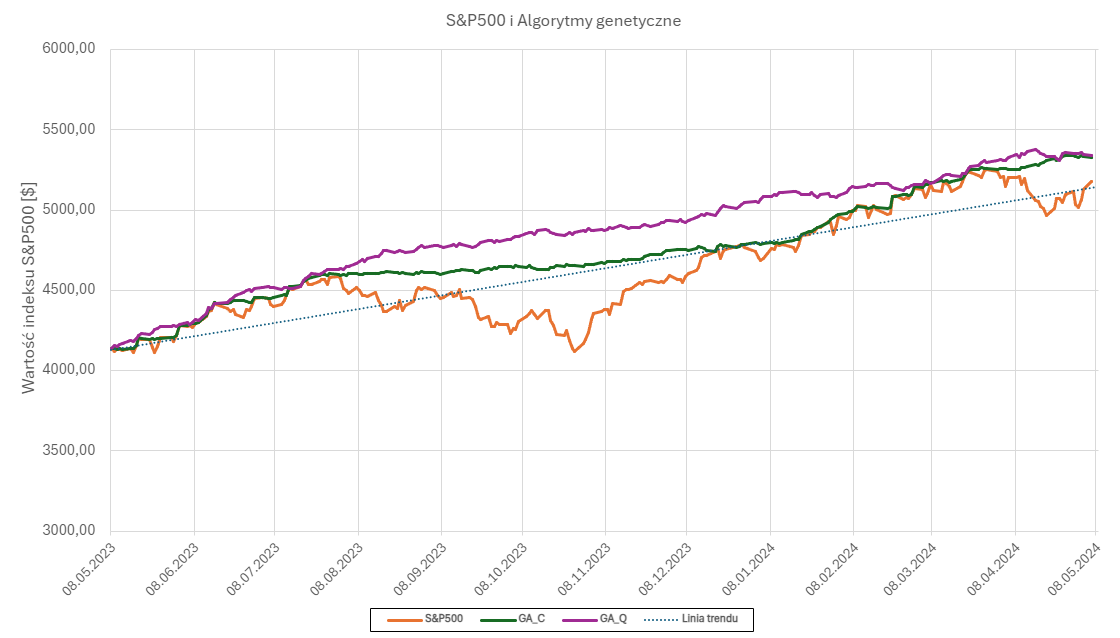
\includegraphics[width=0.8\textwidth]{GA_Q.png}
    \caption{Zestawienie indeksu S\&P500 z graniem na giełdzie z wykorzystaniem algorytmu genetycznego klasycznego i wykorzystującego bramki kwantowe. }
    \label{fig:GA_Q}
\end{figure}

\subsection{Wnioski}

Zarówno algorytm genetyczny klasyczny, jak i wykorzystujący bramki kwantowe, pozwalają na uzyskanie wyniku zbliżonego do zadanego indeksu. Lekkie wyprzedzenie indeksu wynika ze stochastycznej natury tych algorytmów, próbujących przez swą naturę znaleźć najbardziej odpowiadający portfel akcji.

\section{Wnioski}

\subsection{Projekt badań}

\begin{itemize}
    \item \textbf{Potencjał innowacyjny:} Projekt nad kwantowym algorytmicznym handlem ujawnia obiecujący potencjał wykorzystania zaawansowanych technologii obliczeniowych w sektorze finansowym. Eksploracja tego obszaru może prowadzić do nowych perspektyw w zarządzaniu portfelem inwestycyjnym oraz strategiach handlowych.
    
    \item \textbf{Wymóg interdyscyplinarności:} Badanie kwantowych strategii handlowych wymaga synergii wiedzy z różnych dziedzin, w tym finansów, informatyki kwantowej i statystyki. Współpraca między specjalistami z tych obszarów jest kluczowa dla skutecznego przeprowadzenia projektu.
    
    \item \textbf{Zastosowanie zaawansowanych technologii:} Projekt ten stawia przed nami wyzwanie w zakresie zaawansowanych umiejętności programistycznych oraz potrzeby korzystania z nowoczesnych narzędzi obliczeniowych. Konieczne jest pełne zrozumienie skomplikowanych mechanizmów matematycznych i rynkowych.
    
    \item \textbf{Wyzwania i ograniczenia:} Opracowanie kwantowych strategii handlowych wymaga rozwiązania szeregu technicznych, metodologicznych i danych wyzwań. Konieczne jest uwzględnienie ewentualnych ograniczeń technologicznych oraz metodologicznych, aby zapewnić wiarygodność i rzetelność wyników.
    
    \item \textbf{Potencjał publikacyjny:} Wyniki naszych badań mogą stanowić wartościowy wkład w literaturę naukową z zakresu finansów i informatyki kwantowej. Istnieje potencjał publikacji naszych rezultatów w renomowanych czasopismach naukowych oraz prezentacji na prestiżowych konferencjach branżowych.
\end{itemize}

\subsection{Studium pilotażowe}


\section{Literatura}

\end{document}

